%% Keywords usadas: (graphic processing unit or GPU) and (lighting or light or shadow*)

\chapter{Análise Bibliográfica sobre Graphics Processing Unit, por Gustavo Tomás}

\section{Planejamento do estudo}

O objetivo do trabalho é analisar o impacto e popularização das tecnologias utilizadas pelas GPUs (Graphic Processing Units) no processamento e simulação da luz. Para isso, foram utilizadas as ferramentas Bibliometrix e Biblioshiny. Algumas perguntas para basear a pesquisa são:

\begin{itemize}
    \item Como se deu o crescimento das pesquisas sobre GPUs com o passar dos anos?
    \item Quais autores possuem o maior impacto nesses campos de pesquisa?
\end{itemize}

\subsection{Limitações} O exercício relatado foi feito em cerca de uma semana, entre os dias 02 e 10 de fevereiro de 2022 e a base de dados utilizada foi Web Of Science (WoS).

\section{Coleta de dados}

A coleta de dados foi feita usando o WoS no dia 04/02/2022, por meio do Portal de Periódicos da CAPES. Foram feitas buscas nas coleções Science Citation Index Expanded (SCI-EXPANDED) e Social Sciences Citation Index (SSCI), mas com o foco em registros relativos a área de ciências naturais e exatas. A busca utilizada foi a seguinte:

\begin{verbatim}
(graphic processing unit or GPU) 
and
(lighting or light or shadow*)
\end{verbatim}

Essa busca consiste em dois termos, sendo que o primeiro é composto pela GPU (por extenso ou pela sigla) e o segundo pelas palavras luz ou iluminação ou sombra(s). Dessa forma, foram encontrados 1311 registros, sendo que nesse trabalho foram utilizados os primeiros 1000 registros. Esse dataset doravante será chamado de db\_GPU.

\section{Análise dos dados}

\subsection{Filtragem de registros}
Antes da análise, foram aplicados filtros aos registros, de forma que apenas registros do tipo \textit{article}, de qualquer ano e com qualquer número de citações, fossem analisados. O resultado consiste em 850/1000 registros originais.

\subsection{Análise descritiva do dataset}

As informações mais gerais sobre o \textit{dataset} são as seguintes:
\begin{description}
    \item  [\textit{Timespan}] Os artigos analisados foram publicados entre os anos de 1992 e 2022.
    \item  [\textit{Sources}] O dataset é composto por 360 fontes diferentes (dentre artigos, livros e outros).
    \item 
    [\textit{Average years from publication}] A média do tempo de publicação é de 6 anos.
    \item 
    [\textit{Average citations per document}] Cada artigo no dataset foi citado em média 18.55 vezes.
    \item 
    [\textit{References}] O dataset contém 27463 referências citadas.
\end{description}

\subsection{Evolução da Produção Científica}

O gráfico em \ref{fig:gpu-prod-cient} apresenta a evolução da produção científica, mostrando uma forte tendência de crescimento a partir de 2007.

\begin{figure}[ht]
    \centering
    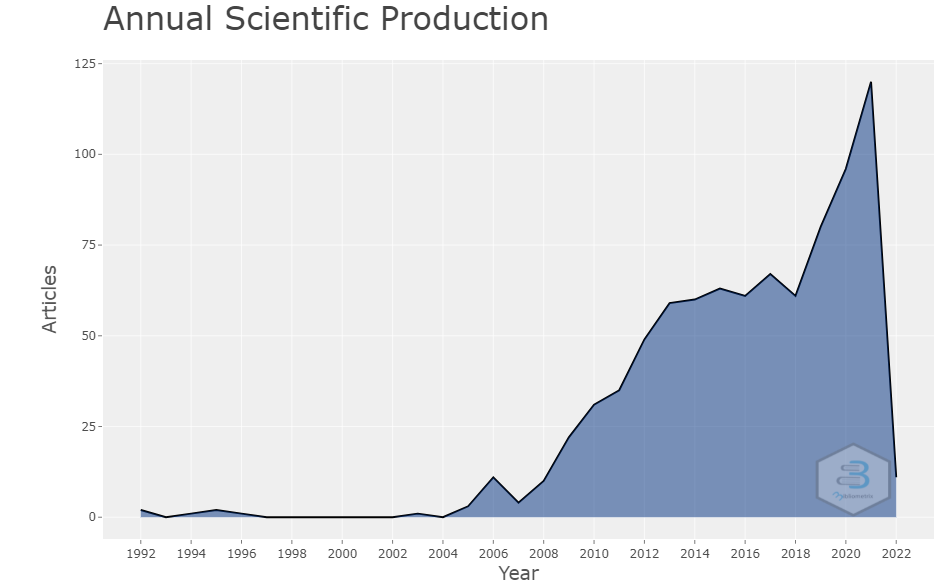
\includegraphics[width=12cm]{experiments/gustavo-tomas/AnaliseBibliometrica/GPUs/Graficos/gpu-prod-cient.png}
    \caption{Evolução da produção científica presente no \textit{db\_GPU}}
    \label{fig:gpu-prod-cient}
\end{figure}

O gráfico mostra um enorme crescimento na área, com destaque ao ano de 2021 com 120 documentos produzidos, um crescimento de 25\% em relação ao ano de 2020.

Nos anos de 2019-2021, em particular, foram introduzidas novas placas de vídeo no mercado, com poder computacional bem maior que as anteriores (é possível comparar as placas 1080 com as gerações 2080 e 3080 e perceber um aumento substancial de qualidade).

\subsection{Evolução das Citações}

A figura em \ref{fig:gpu-citation-year} mostra o número de citações médias feitas por ano. Nota-se uma grande quantidade de citações no ano de 2007, provavelmente devido a um artigo muito citado por outros autores. Nota-se também o que em uma faixa de 20 anos (1992-2021) o número de citações por ano aumentou de 0.2 para 1.0, um aumento de 5 vezes.

\begin{figure}[ht]
    \centering
    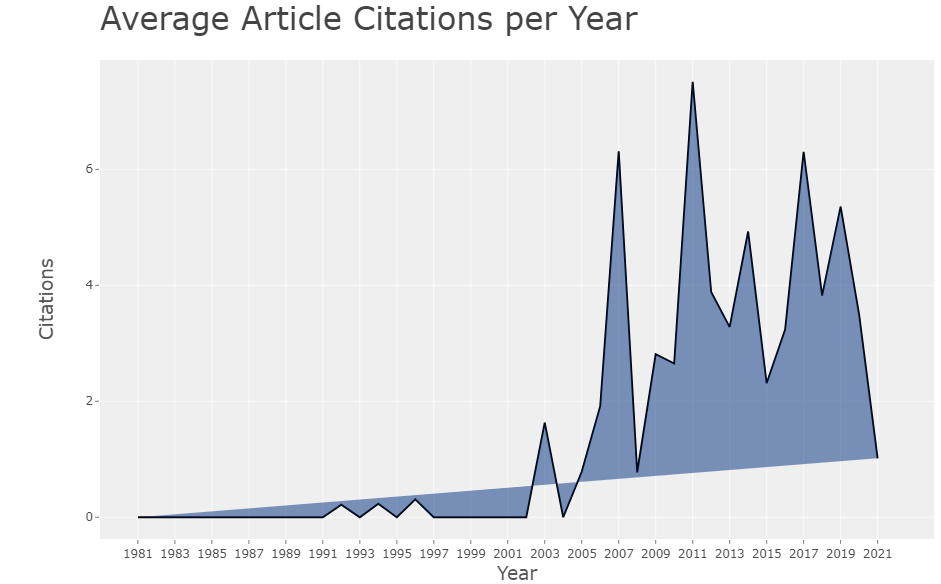
\includegraphics[width=12cm]{experiments/gustavo-tomas/AnaliseBibliometrica/GPUs/Graficos/gpu-citation-year.png}
    \caption{Evolução das citações por ano no \textit{db\_GPU}}
    \label{fig:gpu-citation-year}
\end{figure}

\subsection{\textit{Gráfico de três campos}}

O gráfico em \ref{fig:gpu-three-field} mostra um gráfico de três campos feitos com os dados acerca das referências, autores e palavras-chaves mais relevantes.

\begin{figure}[ht]
    \centering
    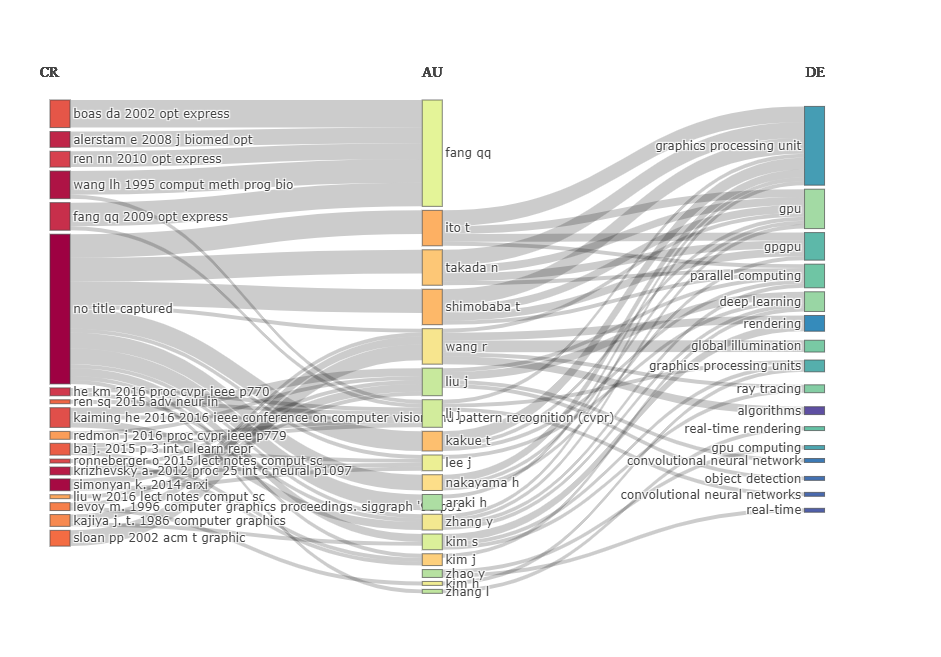
\includegraphics[width=12cm]{experiments/gustavo-tomas/AnaliseBibliometrica/GPUs/Graficos/gpu-three-field.png}
    \caption{Gráfico de três campos analisando palavras-chave no \textit{db\_GPU}}
    \label{fig:gpu-three-field}
\end{figure}

Observando as palavras-chaves, é possível perceber que termos como iluminação, processamento em paralelo e \textit{ray tracing} são expressões relevantes no contexto de GPUs.

Em particular, a técnica de \textit{Ray Tracing} foi otimizada nos últimos anos, de forma que é possível aplicá-la em simulações em tempo real (que antes não era possível devido ao alto custo computacional).

Observando os autores é possível perceber que a maior parte é de origem asiática e que esses autores utilizam principalmente \textit{masuda n 2006 opt express} como referência.

Essa publicação em específico relata avanços feitos na redução do custo computacional para geração de hologramas (objetos tridimensionais) em ambientes computacionais.

\subsection{Refinamento da coleta de dados}

O gráfico em \ref{fig:gpu-co-occur} mostra a rede de co-ocorrências de palavras-chave no \textit{db\_GPU}. Dentro os termos é possível perceber que os assuntos tratados são relevantes ao tópico de GPUs, com destaque ao campo em verde que separa assuntos relativos a dispersão de luz em meios turbulentos (\textit{turbid media}).

\begin{figure}[ht]
    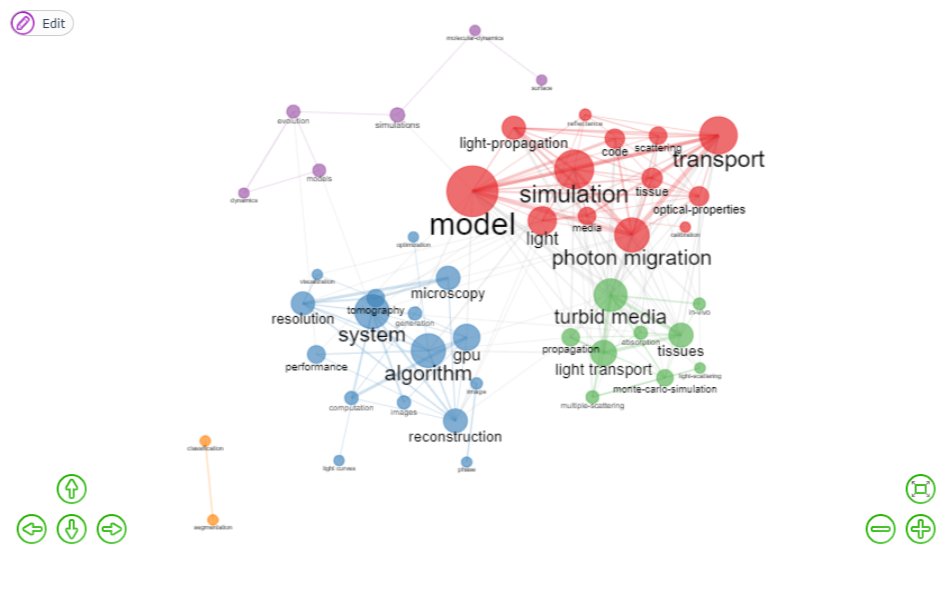
\includegraphics[width=12cm]{experiments/gustavo-tomas/AnaliseBibliometrica/GPUs/Graficos/gpu-co-ocurr.png}
    \caption{Rede de co-ocorrências de palavras-chave no \textit{db\_GPU}}
    \label{fig:gpu-co-occur}
\end{figure}

Esses tópicos são de especial interesse ao tópico de simulação de luz, pois essa simulação se dá por meio de aproximações ao mundo real (modelos físicos e fórmulas matemáticas). Um modelo eficiente consegue reter a essência dos fenômenos reais, de modo que é possível realizar uma simulação realista com uma capacidade computacional não tão elevada.

Softwares de animação (como blender) e de simulação possuem \textit{engines} que simulam fenômenos físicos, tais como corpos sólidos, emissores, índice de refração de materiais e reflexo da luz. Em especial, a \textbf{simulação de Monte Carlo} permite que uma amostra aleatória de possíveis caminhos de luz convirjam para uma solução correta, tornando esse método um dos métodos físicos mais precisos existentes.
